\documentclass[border=10pt]{standalone}
\usepackage{tikz}
\usetikzlibrary{calc,math}
\usepackage{xcolor}
\begin{document}

% this diagram is based off "planets" by Gerard Fleuter
% <https://texample.net/planets/> and "pascal triangle"
% by M.H. Ahmadi <https://texample.net/pascal-triangle/>

% if using light theme, comment out below:
\pagecolor{black}

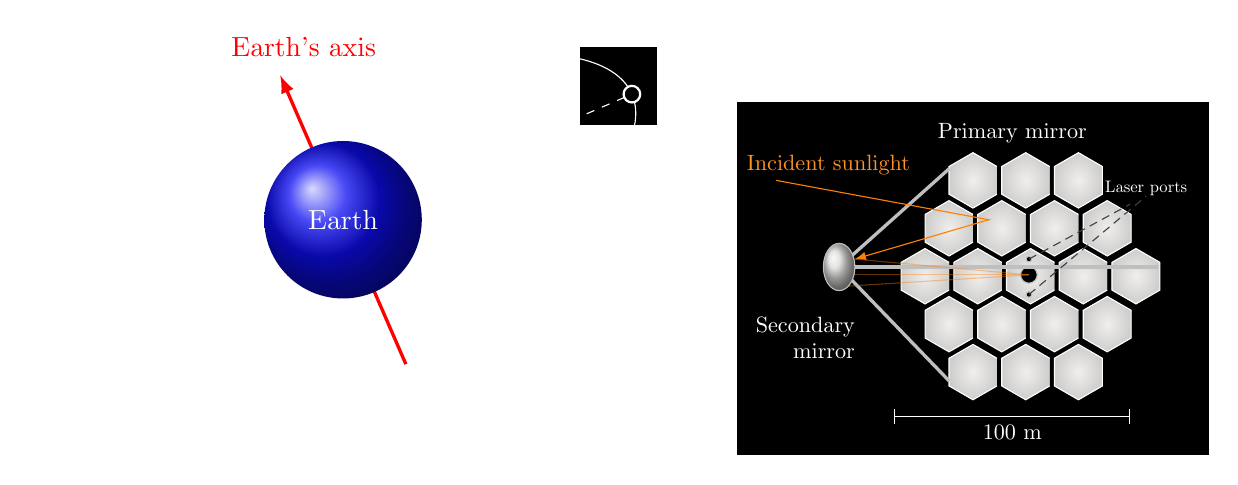
\begin{tikzpicture}[>=latex]
% diagram colors

% custom colors
\definecolor{mirrorSilver}{HTML}{E5E4E2}
\definecolor{mirrorLightsilver}{HTML}{C4C4C4}

% light themed defaults
% \def\primaryColor{black}
% \def\secondaryColor{darkgray}
% \def\bgColor{white}

% dark themed alternatives
\def\primaryColor{white}
\def\secondaryColor{lightgray}
\def\bgColor{black}

% other colors
\def\planetShading{gray!10!blue}
\def\mirrorShadingFill{mirrorSilver!80!mirrorLightsilver}
\def\mirrorShadingOuter{mirrorSilver!90!black}
\def\mirrorShadingInner{mirrorSilver!60!white}
\def\secondaryMirrorShading{gray!10!mirrorSilver}

% begin drawing
    
  % box around spacecraft
  \coordinate (smallboxlowerleft) at (3, 1.2);
  \coordinate (smallboxupperright) at (4, 2.2);
  \draw[\primaryColor, fill=\bgColor, thin] (smallboxlowerleft) rectangle (smallboxupperright);

  %  orbit (Earth's axial tilt is 23.5 degrees)
  \draw[\primaryColor, rotate=23.5] ellipse  (4 and 1.5);
  \draw[\primaryColor, dashed, rotate=23.5] (0,0) -- (4,0);
  \node[\primaryColor, align=right] at (1.5, 1.2) {35,786 km};
  \node[\primaryColor] at (-0.5, -2.5) {\textbf{Geostationary orbit}};

  % earth axis
  \draw[->, very thick, color=red, rotate=23.5] (0,-2) -- (0,2);
  \node[text=red, align=right] at (-0.5, 2.2) {Earth's axis};

  % earth
  \shade[ball color=\planetShading] circle (1);
  \node[text=white] (earth) {Earth};

  % spacecraft
  \filldraw [\primaryColor, fill=\bgColor, rotate=23.5, thick] (4, 0) circle (3pt);

  % expanded box
  \coordinate (bigboxlowerleft) at (5,-3);
  \coordinate (bigboxupperleft) at (5,1.5);
  \draw[\primaryColor] (smallboxlowerleft) -- (bigboxlowerleft);
  \draw[\primaryColor] (smallboxupperright) -- (bigboxupperleft);
  \draw[\primaryColor, fill=\bgColor, thin] (bigboxlowerleft) rectangle (11,1.5);

    % mirrors
    % Draws a row of compound mirrors
    % first argument is the number of mirrors in a row
    % second and third are the x- and y-shifts
    \newcommand\mirrorRow[3]{
        \newdimen\R
        \R = 10pt
        \begin{scope}[shift={({-sqrt(3)/2 *\R*#2},{-sqrt(3)*\R*#3})}]
        % draw submirrors column-wise across each row
        \pgfmathtruncatemacro\cols{#1 - 2}
        \foreach \j in {0,...,\cols} {
            % the factor of 1.1 is to space out things a little
            \begin{scope}[shift={({1.1*sqrt(3)*\R*\j},0)}]
                 % draw open hexagons (the right edge
                 % isn't closed to prevent double-drawing)
                \draw[\primaryColor, 
                      fill=\mirrorShadingFill,
                      outer color=\mirrorShadingOuter,
                      inner color=\mirrorShadingInner
                      ] (30:\R) \foreach \x in {90,150,...,330} { 
                    -- (\x:\R) };
            \end{scope}
        }
        % last hexagon on each row should be closed
        \draw[\primaryColor, 
              fill=\mirrorShadingFill,
              outer color=\mirrorShadingOuter,
              inner color=\mirrorShadingInner,
              % the factor of 1.1 is to space out things a little
              shift={({1.1*sqrt(3)*\R*(#1 - 1)},0)}] (30:\R) \foreach \x in {90,150,...,330} { 
            -- (\x:\R) } --cycle;
        \end{scope}
    }


\begin{scope}[shift=({8,0.5})]
% primary mirror
\mirrorRow{3}{0}{0}
\mirrorRow{4}{1}{1}
\mirrorRow{5}{2}{2}
\mirrorRow{4}{1}{3}
\mirrorRow{3}{0}{4}

% light outlet
\coordinate (lightIncident) at (-2.5,0);
\coordinate (outletPos) at (0.71,-1.2);
\coordinate (outletOffsetUpper) at (0.71,-1);
\coordinate (outletOffsetLower) at (0.71,-1.45);
\draw[\secondaryColor, fill=\bgColor] (outletPos) circle (3pt);
% additional outlets for maser
\draw[\secondaryColor, fill=\bgColor] (outletOffsetLower) circle (1pt);
\draw[\secondaryColor, fill=\bgColor] (outletOffsetUpper) circle (1pt);

% secondary mirror coordinates
\coordinate (leftattachment) at (-0.3, 0.15);
\coordinate (rightattachment) at (2.35, -1.1);
\coordinate (bottomattachment) at (-0.3, -2.55);
\coordinate (secondarymirrorpivot) at (-1.7,-1.1);
\coordinate (primaryfocus) at (-1.6,-1);
\coordinate (primaryfocusOffset) at (-1.5,-1);

% attachment spokes of secondary mirror
% uncomment below to see visual markers of the
% attachment points
% \filldraw [\primaryColor, fill=\bgColor, rotate=23.5, thick] (leftattachment) circle (3pt);
% \filldraw [\primaryColor, fill=\bgColor, rotate=23.5, thick] (rightattachment) circle (3pt);
% \filldraw [\primaryColor, fill=\bgColor, rotate=23.5, thick] (bottomattachment) circle (3pt);
% \filldraw [\primaryColor, fill=\bgColor, rotate=23.5, thick] (secondarymirrorpivot) circle (3pt);
\draw[\secondaryColor, very thick] (leftattachment) -- (secondarymirrorpivot);
\draw[\secondaryColor, very thick] (rightattachment) -- (secondarymirrorpivot);
\draw[\secondaryColor, very thick] (bottomattachment) -- (secondarymirrorpivot);

% focused light
\draw[->, color=orange] (lightIncident) -- (0.2,-0.5) -- (primaryfocusOffset);
\node[text=orange!85!\primaryColor, text width=3cm, align=right, scale=0.8] at (-2, 0.2) {Incident sunlight};
\draw[color=orange,opacity=0.4] (-1.5,-1) -- (outletPos);
\draw[color=orange,opacity=0.4] (-1.55,-1.2) -- (outletPos);
\draw[color=orange,opacity=0.4] (-1.7,-1.35) -- (outletPos);

% secondary mirror
%\draw[fill=\bgColor] (secondarymirrorpivot) ellipse (0.2 and 0.3);
\shade[ball color=\secondaryMirrorShading] (secondarymirrorpivot) ellipse (0.2 and 0.3);
\draw[\secondaryColor] (secondarymirrorpivot) ellipse (0.2 and 0.3); % secondary mirror outline

% labels
\node[text=\primaryColor] at (0, 1.5) {\textbf{Solar mirror}};
\node[text=\primaryColor, scale=0.8, align=left] at (0.5, 0.6) {Primary mirror};
\node[text=\primaryColor, scale=0.8, text width=2cm, align=right] at (-2.3, -2) {Secondary mirror};
\draw[|-|, \primaryColor] (-1, -3) -- (2, -3);
\node[scale=0.8, \primaryColor] at (0.5,-3.2) {100 m};
\draw[darkgray, densely dashed] (outletOffsetLower) -- (2.2,-0.2);
\draw[darkgray, densely dashed] (outletOffsetUpper) -- (2,-0.3);
\node[text=\primaryColor, scale=0.6] at (2.2, -0.1) {Laser ports};

\end{scope}

\end{tikzpicture}
\end{document}